\section{DQL: empty goal}\label{DQL}

We train the RL gfootball empty goal setting, using Adam optimizer, learning rate of 0.001.

At the heart of the DQL model, we build a 2-layers Neural Net, with 24+48 nodes and Relu activation. We update it at every step after updating the Q-value for given state-action pair.

The model is compiled in Google Colab.

To test learning, we examine the loss function. We plot the loss function as function of episodes, see figure \ref{fig_dql_loss}. We also plot the number of steps before ``done'' in figure \ref{fig_dql_steps}, and rewards as a function of episodes.


\begin{center}
%\begin{tabular}{lclc}
%(a) &
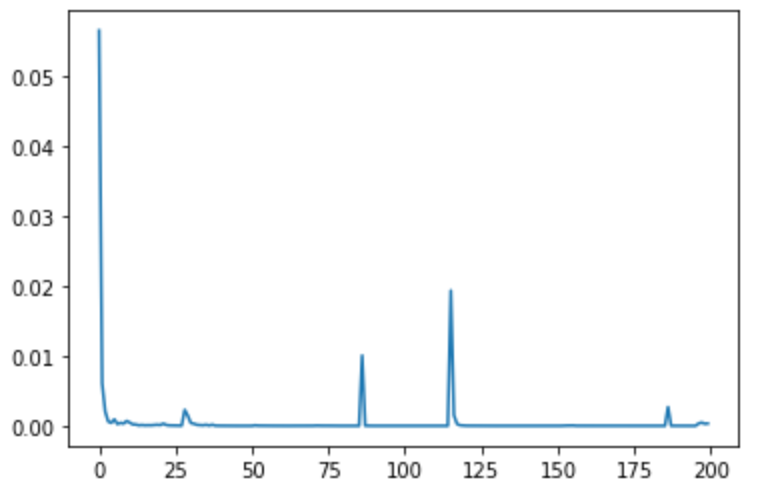
\includegraphics[width=5cm]{fig_dql_loss.jpg}
%& (b)
%&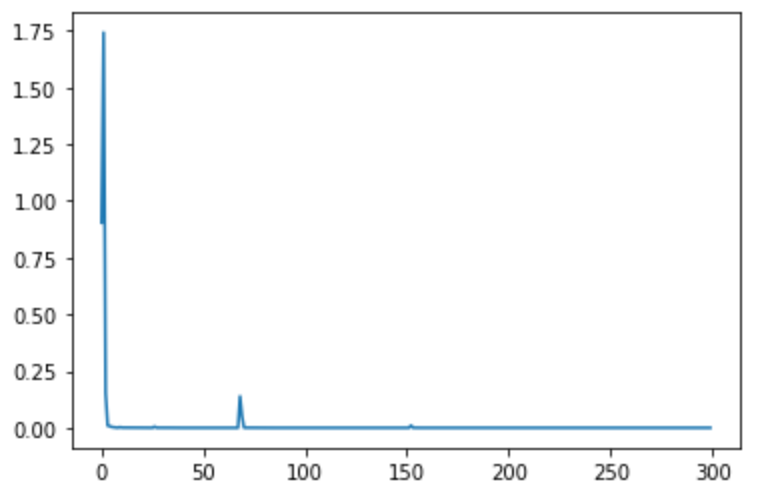
\includegraphics[width=5cm]{fig_dql_loss_long.jpg}
%\end{tabular}
\captionof{figure}{DQL model training loss.}
\label{fig_dql_loss}
\end{center}


\begin{center}
%\begin{tabular}{lclc}
%(a) &
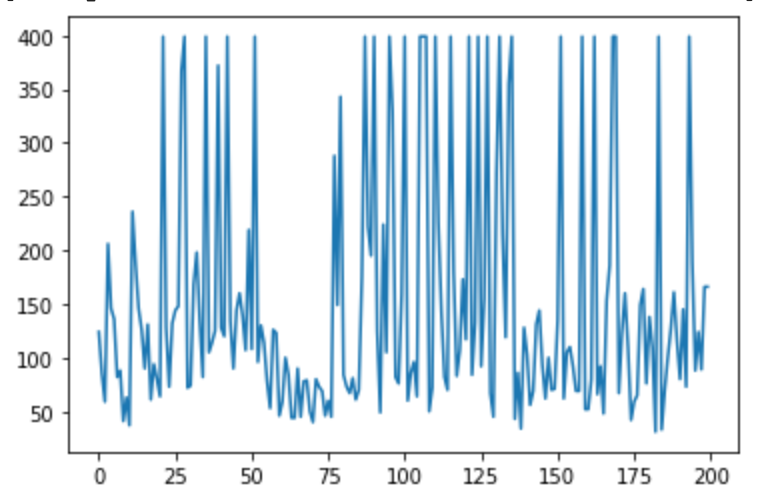
\includegraphics[width=5cm]{fig_dql_steps.jpg}
%& (b)
%&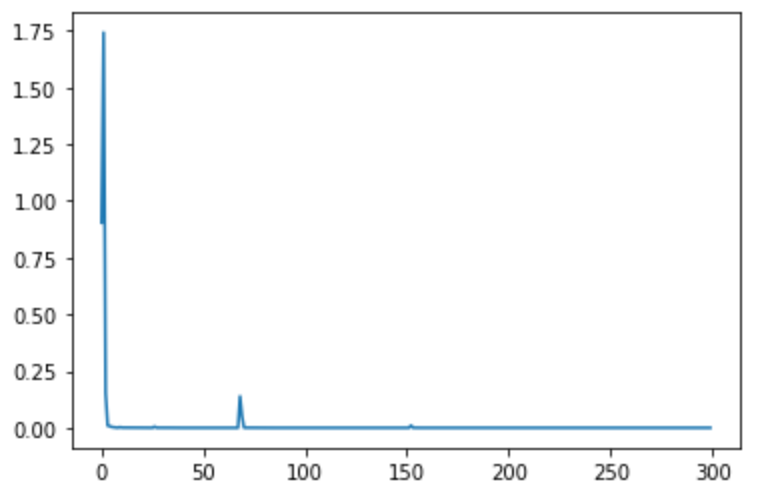
\includegraphics[width=5cm]{fig_dql_loss_long.jpg}
%\end{tabular}
\captionof{figure}{DQL model steps before ``done''.}
\label{fig_dql_steps}
\end{center}